\section{Optimization Methodology}
We now present the optimization function, parameters and assumptions to tune SQL-on-Hadoop data engines. Even though the model is specific to run time features of SQL-on-Hadoop engines, the principles can be translated to other engines. 

\subsection{Optimization Function}
The optimization function should consider both cost and performance of a workload. In this section, we develop a metric to capture cost and performance of SQL-on-Hadoop engines running on Hadoop2 Yarn Containers. Hadoop divides machines into containers and each container is assigned a fixed amount of memory and CPUs (can be fractional). Workloads are submitted to Hadoop by Hive or Spark. Hadoop schedules tasks on containers. 
The cumulative time that a workload is scheduled on all the containers is a good proxy for the cost of the query. Therefore the cost of a query is $\mathcal{T} = \sum_{i=1}^{n} t_i$ where $n$ is number of containers and $t_i$ is execution time for $i^{th}$ container. The time factor in the equation tracks the performance of the query.

\subsection{Parameters}
From OtterTune \cite{VanKen}, a tool to auto tune Databases like MySQL and PostGres it was found that tuning only few knobs can improve performance significantly. We used this finding to choose few parameters by consulting experts in the domain. Following are the parameters of the model which would be used in the first algorithm:
\begin{enumerate}
    \item[$\bullet$] Job Parameters: There are the input parameters of the job that needs to be specified. Table \ref{table:job_params} defines these job parameters.
    \item[$\bullet$] Instance configuration: Table \ref{table:inst_conf} defines the machine configuration.
    \item[$\bullet$] Global Parameters: These are some of the global parameters that can be used to tune the algorithm. These are defined in Table \ref{table:global_params}.
\end{enumerate}

\begin{table}
\begin{tabular}{ |l|p {4.5 cm}| } 
 \hline
 Parameters & Description \\ 
 \hline
 mapperTime  & Total mapper time in seconds   \\ 
 numOfMapper & Number of map tasks \\ 
 mapperMemory & Container memory for map tasks  \\ 
 splitSize & Input Split Size \\
 mapperOutputBytes & Map output in bytes \\
 mapperOutputRecords & Number of Map output records \\
 reducerTime & Total reducer time in seconds \\
 numOfReducer & Number of reduce tasks \\
 bytesPerReducer & Corresponds to Hive parameter \textit{hive.exec.reducers.bytes.per.reducer} \\
 reducerMemory & Container memory for reduce tasks \\
 ioSort & Total amount of buffer memory in mega bytes to be used for sorting. Corresponds to Hadoop parameter \textit{mapreduce.task.io.sort.mb} \\
 spilledMapRecords & Number of records spilled in Map tasks  \\
 \hline
\end{tabular}
\caption{Parameters of the Job to be optimized}
\label{table:job_params}
\end{table}

\begin{table}
\begin{tabular}{ |l|p {4.5 cm}| }
 \hline
 Parameters & Description \\ 
 \hline
 nodeMemory  & Total available memory per node for MR job   \\ 
 cpuPerNode & Number of CPUs per node \\ 
 vCpuPerNode & Number of vCPUs per node  \\ 
 \hline
\end{tabular}
\caption{Instance configuration}
\label{table:inst_conf}
\end{table}

\begin{table}
\begin{tabular}{ |p {1.5 cm}|p {3.5 cm}|p {1 cm} | } 
 \hline
 Parameters & Description & Default\\ 
 \hline
 ioSortFrac & Size of ioSort buffer specified as fraction of mapper memory & 0.4 \\
 maxIOSort & Maximum value for \textit{mapreduce.task.io.sort.mb} & 2047 \\
 \hline
\end{tabular}
\caption{Global Parameters}
\label{table:global_params}
\end{table}

For Map-Reduce engine, the parameters are described in Tables 1, 2 and 3.

\subsection{Assumptions}

\begin{figure*}[h]
	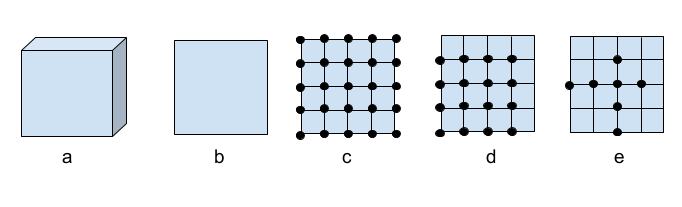
\includegraphics[width=\linewidth]{fig/searchspace.png}
	%\vspace*{-15pt}
	\caption{Reducing the search space}
	\label{fig:searchspace}
\end{figure*}


\noindent\subsubsection*{\bf Reducing the search space: }
The main challenge in such methods is to limit the number of trials, since each execution takes up resources and has a monetory cost associated with it. Earlier approaches based on iterative execution have used various techniques such as noisy gradient~\cite{} to converge to a solution faster. In our method, we make use of domain knowledge and heuristics to reduce the search space. Specifically, we employed the following strategies to reduce the parameter space to be explored.

\noindent\subsubsection*{\bf Parameter reduction: }
+\label{sec:paramreduction}
The search space is exponential in the number of parameters to be optimized. As described earlier, there are a large number of paramerters that can be set for any hive query. However, based on the experience of tuning a large number of real customer workloads, we can identify a smaller set of parameters that have a relatively larger impact on the performance of sql queries. We restrict the search to these parameters, thus reducing the search space. These parameters have been listed in Table~\ref{}. The search space with a restricted set of parameters is shown in Figure~\ref{fig:searchspace}(a).
\noindent\subsubsection*{\bf Discretization: }
Each parameter, such as memory or partition size, can take a large number of values. However, it can be observed that small changes in the parameters do not have a significant impact. Thus, instead of trying each possible value, it is sufficient to discretize the parameter range and consider only a subset of values for each parameter. These values are placed at a reasonbale distance from each other so as to hvae a significant impact on the query performance. For example, instead of varying memory in units of 1 MB, we can vary it in multiples of 128 MB. The resulting search space is shown in Figure~\ref{fig:searchspace}(b).
\noindent\subsubsection*{\bf Range reduction: }
The range of values for each parameter is further restricted based on domain knowledge about what a good range for that parameter would be.  The knowledge about a good range can be gained by either talking to experts or by looking at some other metrics. For example, for the Hive on MR engine, consider the mapper\_time metric that measures the average time taken by a mapper. If the mapper time is too low, the overhead of starting the mappers is large compared to the actual work done by the mapper. Since the mapper time is inversely related to the number of mappers, the number of mappers need to be reduced. On the other hand, if the mapper time is large, then the job parallelism is restricted and the end to end clock time taken for the query will be high. In this case, more mappers are needed to reduce the work that each mapper has to do. A good acceptable range for this metric could be from 240s till 1800s.  If a set of config params results in mapper\_time beyond the acceptable range, it should not be considered in the search process. For example, mapper\_time is affected by mapreduce.input.fileinputformat.split.maxsize and the correlation is direct, i.e. mapper\_time  increases as we increase mapreduce.input.fileinputformat.split.maxsize.  Thus the split maxsize should be constrained to a range that will lead to a reasonable mapper\_time. In our experiments, we restricted splitsize to between 128 MB and 1 GB. The resulting search space is shown in Figure~\ref{fig:searchspace}(c).
\noindent\subsubsection*{\bf Dimension independence: } 
We make an assumption that the parameters are not correlated to each other. This enables us to optimize each parameter independently of the others. Thus, rather than exploring all the points in the search space, the algorithm explores only one set of values for each parameter as show in Figure~\ref{fig:searchspace}(d). This is a very strong assumption, which may not hold in practice. For example, the mapper memory (mapreduce.map.memory.mb) and the splitsize (mapreduce.input.fileinputformat.split.maxsize) are correlated, since more memory is needed by the mappers as the splitsize increases if spills are to be avoided. Even in this case, the algorithm will find the best value for memory after fixing the splitsize or the best splitsize after fixing the memory. So overall the configuration chosen will be a reasonably good one.
